% !TeX TXS-program:compile = txs:///pdflatex/[--shell-escape]
\documentclass[handout, aspectratio=169, 10pt]{beamer}

% packages
\usepackage{newpxmath} % math font is Palatino compatible
% \usepackage[nomath]{fontspec}

\usepackage{setspace}
\usepackage{xcolor}
\usepackage{soul} % for \st
\usepackage{hyperref} % for links
\definecolor{links}{HTML}{2A1B81}
\hypersetup{colorlinks,linkcolor=,urlcolor=links}


% table stuff
\usepackage{chronosys}
\usepackage{verbatim}
% \pagenumbering{arabic}
\usepackage{tabularx}
\usepackage{booktabs}
\usepackage{ragged2e}
\usepackage{mathtools}

% R Code
\usepackage{listings}
\usepackage{courier}
\lstset{basicstyle=\scriptsize\ttfamily,breaklines=true}
\lstset{framextopmargin=50pt,frame=bottomline}

% themes
\usetheme[progressbar=frametitle, block=fill]{metropolis}
\useoutertheme{metropolis}
\useinnertheme{metropolis}

% colors
\definecolor{dimwhite}{rgb}{0.99, 0.99, 0.99}
\definecolor{charcoal}{rgb}{0.21, 0.27, 0.31}
\definecolor{slategray}{rgb}{0.44, 0.5, 0.56}
\definecolor{dimgray}{rgb}{0.41, 0.41, 0.41}
\definecolor{bleudefrance}{rgb}{0.19, 0.55, 0.91}

% beamer options
\setbeamercolor{author}{fg=charcoal}
\setbeamercolor{background canvas}{bg=white}
\setbeamercolor{section in toc}{fg=charcoal}
\setbeamercolor{subsection in toc}{fg=dimgray}
\setbeamercolor{frametitle}{bg=dimwhite, fg=charcoal}
\setbeamercolor{progress bar}{fg=slategray, bg=fg!50!black!30}
\setbeamercovered{transparent}
\setbeamertemplate{itemize items}[triangle]
\setbeamertemplate{itemize subitem}[circle]
\setbeamertemplate{itemize subsubitem}[square]
\setbeamersize{text margin left=7mm,text margin right=7mm} 

% new commands
\newcommand{\q}[1]{``#1''}
\newcommand{\hs}[1]{\textsc{\hfill\scriptsize\color{dimgray}#1}}
\newcommand{\g}[1]{{\color{gray}#1}}
\newcommand{\dg}[1]{{\color{dimgray}#1}}
\newcommand{\sg}[1]{{\color{slategray}#1}}
\newcommand{\bdf}[1]{{\color{bleudefrance}#1}}
\newcommand{\itemcolor}[1]{\renewcommand{\makelabel}[1]{\color{#1}\hfil ##1}}
\newcommand\Wider[2][2em]{
\makebox[\linewidth][c]{
  \begin{minipage}{\dimexpr\textwidth+#1\relax}
  \raggedright#2
  \end{minipage}
  }
}

% misc
\linespread{1.35}

% minted (risky)
\usepackage[cache=false]{minted}

% Math stuff
\newcommand{\norm}[1]{\left\lVert#1\right\rVert}
\newcommand{\R}{\mathbb{R}}
\newcommand{\E}{\mathbb{E}}
\newcommand{\V}{\mathbb{V}}
\newcommand{\probP}{\text{I\kern-0.15em P}}
\newcommand{\ol}{\overline}
%\newcommand{\ul}{\underline}
\newcommand{\pp}{{\prime \prime}}
\newcommand{\ppp}{{\prime \prime \prime}}
\newcommand{\policy}{\gamma}
\newcommand{\plim}{ \overset{p}{\to}}
\newcommand{\hnot}{ \overset{H_0}{\to}}

% Causal Graphs
\usetikzlibrary{shapes,decorations,arrows,calc,arrows.meta,fit,positioning}
\tikzset{
    -Latex,auto,node distance =1 cm and 1 cm,semithick,
    state/.style ={ellipse, draw, minimum width = 0.7 cm},
    point/.style = {circle, draw, inner sep=0.04cm,fill,node contents={}},
    bidirected/.style={Latex-Latex,dashed},
    el/.style = {inner sep=2pt, align=left, sloped}
}
\setbeamersize{text margin left=10pt,text margin right=10pt}

\begin{document}


\title[L4 - Inference and Standard Errors]{ Econometrics I}
\subtitle{Lecture 4: Inference and Standard Errors}
\author{Chris Conlon}
\date{Fall 2025}
\maketitle



\begin{frame}{Hypothesis testing}
\begin{itemize}
	\item We are often interested in testing theories, or testing hypotheses about
	the values of certain parameters

	\medskip
	\item Simplest example: testing whether mean of a variable $\mu_x \equiv E\left[X\right]$ 
	is different from a particular value:\[
\begin{array}{c}
H_{0}:\qquad\mu_{x}=a\\
H_{1}:\qquad\mu_{x}\ne a
\end{array}
\]

	\medskip
	\item A hypothesis test typically involves a {\bf null hypothesis} and {\bf alternative hypothesis}. 
	The alternative hypothesis could also be about a particular value ($H_{1}:\mu_{x}= b$, or 
	a one-sided rejection of the null ($H_{1}:\mu_{x}>a$).


\end{itemize}
\end{frame}



\begin{frame}{Review: z test}
\begin{itemize}
	\item If $X_i$ is i.i.d. normal with \emph{known} variance $\sigma^2$, then \[
		\overline{X} \sim \mathcal{N} \left( \mu_x, \sigma^{2}/n \right)
	\]


	\item In this case, we know the distribution of our estimate $\overline{X}$. We can test\[
H_{0}:\mu_{x}=a \qquad H_{1}:\mu_{x}\ne a
\]
using a {\bf z test}.

	\item We construct the test statistic, which under the null hypothesis has the standard normal distribution:
	\begin{align*}		z = \frac{ \overline{X} - a}{n^{-1/2}\sigma}
	 \overset{d}{\to} \mathcal{N} \left( 0,1\right)
	 \end{align*}
\end{itemize}
\end{frame}



\begin{frame}{Level and Size of Test}
\begin{itemize}
	\item The {\bf size} (or {\bf level}) of a test is the probability of rejection if the null hypothesis is true. 
	\emph{The size is the rate of false positives or type I errors.}

	\item When hypothesis testing, we make it hard to reject the null hypothesis. We typically choose the 
	size of the test to be small (most commonly, .01 or .05).

\end{itemize}
\end{frame}




\begin{frame}{Power of Test}
\begin{itemize}

	\item We typically want to reject only for the outcomes that are least likely under the null
	hypothesis (or relatively more likely under the alternative hypothesis than the null). For
	the z test above, we reject only in the tails of the normal distribution. See: Neyman-Pearson Lemma.
	
	\medskip
	\item Choosing the rejection region appropriately maximizes the test's {\bf power}, the 
	probability of rejecting the null hypothesis when it is indeed false. Power is often harder
	to quantify and not something we typically choose. Power is one minus the rate of
	type II errors (\textbf{false negatives}), or failures to reject the null hypothesis when it is false. 
\end{itemize}
\end{frame}



\begin{frame}{Rejection Region and Power}
\begin{columns}
\begin{column}{0.5\textwidth}
\begin{figure}	
	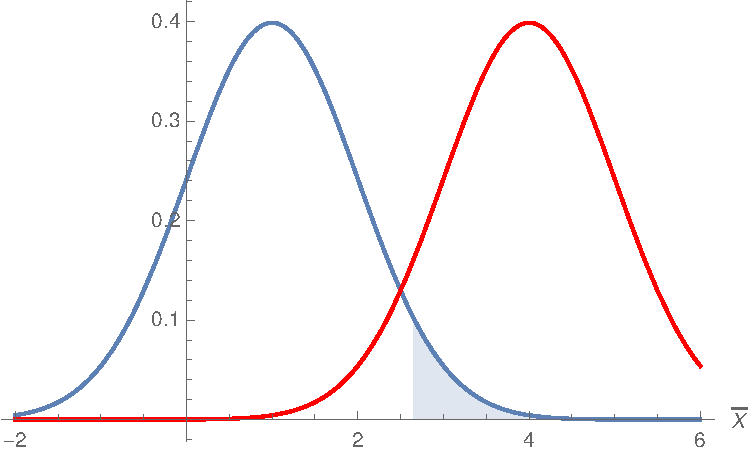
\includegraphics[width=\textwidth]{hypothesis_test.pdf}	
\end{figure}
\end{column}
\begin{column}{0.5\textwidth}
\begin{itemize}
	\item Suppose $\bar{X}$ is normally distributed with $Var\left(\bar{X}\right)=1$ 

	\item We want to test \[
\begin{array}{c}
H_{0}:\qquad\mu_{x}=1\\
H_{1}:\qquad\mu_{x}= 4
\end{array}
\]
	\item The blue and red lines are the PDF of $\bar{x}$ under the null and alternative hypotheses, respectively 

	\item The shaded region is the rejection region with level $\alpha = .05$ that maximizes power. 
	Note that this is for $\bar{X}\ge 2.65$.
	
\end{itemize}

\end{column}

\end{columns}
\end{frame}



\begin{frame}{Rejection Region and Power}
\begin{columns}
\begin{column}{0.5\textwidth}
\begin{figure}	
	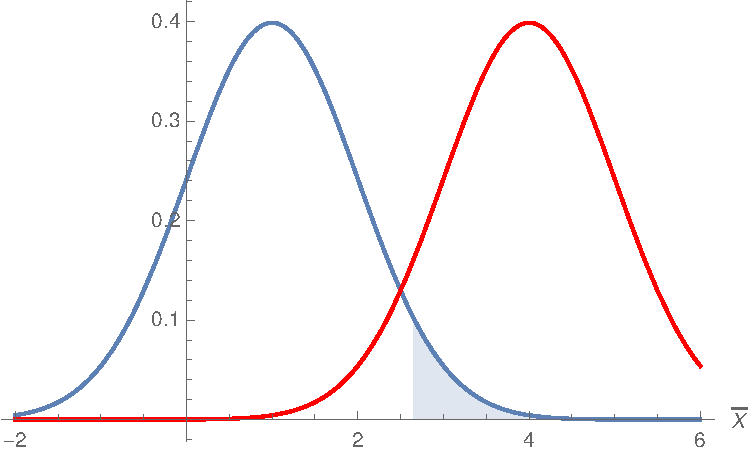
\includegraphics[width=\textwidth]{hypothesis_test.pdf}	
\end{figure}
\end{column}
\begin{column}{0.5\textwidth}
\begin{itemize}
	\item Note that the rejection region is the region where the PDF of
	the alternative hypothesis is high relative to the null hypothesis.
	
	\item The maximum power test with  level $.05$ is the test that rejects for the 5\%
	of the null-hypothesis PDF in which $H_1$'s likelihood (probability density) is highest
	relative to $H_0$'s.

	\item We often take for granted that rejection regions
	are in the tails of the null-hypothesis PDF; this is why.
\end{itemize}

\end{column}

\end{columns}
\end{frame}


\begin{frame}{Review: t Statistics}
\begin{itemize}
	\item Let's return to testing the value of a normally distributed random
	variable's mean, but now let's suppose that $\sigma^2$ is not known (which is
	typically the case).

	\smallskip
	\item Our test statistic instead is\[
		t = \frac{ \overline{X} - a}{n^{-1/2} s}
	\]
	where \[
s=\sqrt{\frac{1}{n-1}\sum_{i=1}^{n}\left(X_{i}-\overline{X}\right)}^2
\]

	\item Here, $t$ has a $t$-distribution with $n-1$ degrees of freedom. 

\end{itemize}
\end{frame}




\begin{frame}{Testing Paradigm}
\begin{itemize}

	\item We focus on different versions of {\bf Wald tests}, which are based on test 
	statistics that are (approximately) normally distributed.

	\medskip
	\item Other paradigms:
	\begin{itemize}
		\item Likelihood Ratio tests and goodness-of-fit-based tests. The idea here is to compare how well
		different models fit the data.

		\item Lagrange multiplier test: for example, testing whether residuals from a restricted model are
		correlated with excluded variables. 
	\end{itemize}
\end{itemize}
\end{frame}


\begin{frame}{Motivating Small Sample $t$-Tests}
\begin{itemize}
	\item Last week we learned that if $N$ is large then,
	\[
		{\bf b}_{OLS} \stackrel{a}{\sim}\mathcal{N}\left(\beta,Var({\bf b}_{OLS})\right)
	\]
	\begin{itemize}
		\item This hinges on knowing $Var({\bf b}_{OLS})$
		\item We rarely know this in practice --- we estimate it instead
		\item Like testing the mean of a normal random variable, estimating the variance
		of the test statistic puts us in a $t$-test situation.
	\end{itemize}
\end{itemize}
\end{frame}

\begin{frame}{$t$-Statistics for OLS Parameters (homoscedasticity)}

\[
\frac{{\bf b}_{OLS,k} - \beta_k}{\sqrt{s^2 \left( {\bf X}' {\bf X}\right)^{-1}_{kk}}} \sim t_{n-K}
\]

\begin{itemize}
	\item where $K$ is the number of parameters,  $s^2$ is the estimator of
	the variance of $\varepsilon$, and \[
	\left( {\bf X}' {\bf X}\right)^{-1}_{kk}
	\]
	refers to the $k$th diagonal element of $\left( {\bf X}' {\bf X}\right)^{-1}$.

	\item Note that the denominator of the above formula is the standard error for the $k$th
	estimated parameter ${\bf b}_{OLS,k} $.

\end{itemize}
\end{frame}


%
%\begin{frame}{The $R^2$ and the Error Variance}
%
%Recall the definition of the $R^2$:
%\[
%	R^2 = \frac{\sum_{i=1}^N (\hat Y_i-\bar Y)^2}{\sum_{i=1}^N(Y_i-\bar Y)^2} = \frac{ESS}{TSS}
%\]
%
%\begin{itemize}
%	\item We call the 	
%\end{itemize}
%
%
%\end{frame}

\begin{frame}{The t-Distribution}

\begin{figure}[htp]
\centering
	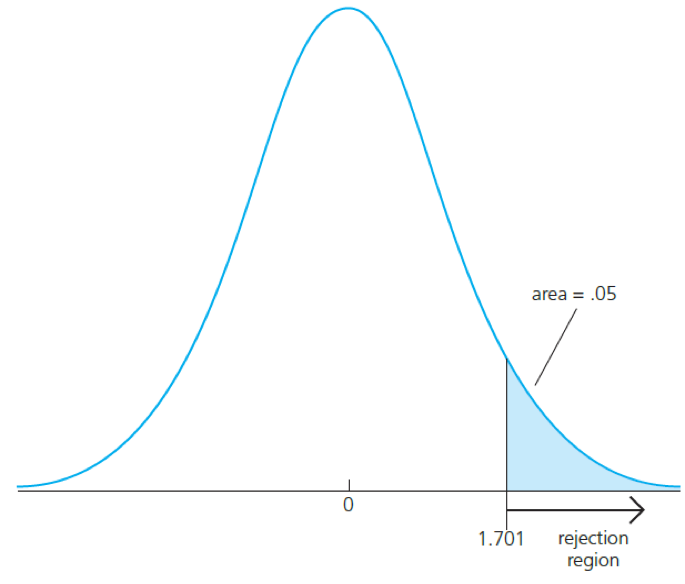
\includegraphics[width=.4\textwidth]{tDistribution}	
\end{figure}

\begin{itemize}
	\item Similar to the $\mathcal{N}(0,1)$ but parametrized by degrees of freedom
	\item The tails are fatter but become $\mathcal{N}(0,1)$ as df go to $\infty$
\end{itemize}
	
\end{frame}

\begin{frame}{Example of Reading a t-Table}
Example of a table of critical values for t distribution from a textbook:
\begin{table}[htp]
\begin{tabular}{ccc}
\hline\hline 
Degrees of Freedom & .10 & .05\\
\hline
1 & 6.31 & 12.71\\
2 & 2.92 & 4.30\\
$\vdots$ & &\\
{\color{red} 28} & 1.70 & {\color{red} \bf 2.05} \\
$\vdots$ & &\\
{\color{red}$\infty$}  & 1.65 & {\color{red} \bf 1.96} \\
\hline
\end{tabular}

\end{table}

\begin{itemize}
	\item If $N$ were very large we would use the $\mathcal{N}(0,1)$ approximation which is exactly the case that $df=\infty$
	\item If $N<\infty$ we can use a table like this, or a computer does it for us
	\item \emph{Example:} If $N=30$, $K=2$, then $df = N-K=28$ the 5\% cutoff value is 2.05 
\end{itemize}

\end{frame}



% HERE

\begin{frame}{An Example (Bivariate Regression)}

\onslide<1->{Suppose I have the following estimated parameters on 30 observations
\begin{align*}
	b_1 =& 1.00\\
	\sum_{i=1}^N(X_i-\bar X)^2 =& 14\\
	\sum_{i=1}^N e_i^2 =& 100
\end{align*}}

\only<2>{
\begin{enumerate}
\item[1.] First, state the hypothesis:
\begin{align*}
	H_0:& \beta_1 = 0\\
	H_1:& \beta_1\ne 0
\end{align*}
\end{enumerate}
}

\only<3>{\begin{enumerate}\item[2.]  Second, calculate $s^2$:
	\begin{align*}
		s^2 =& \frac{1}{N-2}\sum_{i=1}^N( e_i)^2 = 3.45
	\end{align*}
\end{enumerate}
}

\only<4>{\begin{enumerate}\item[3.]  Third, calculate $t$ under $H_0: \beta_1 = 0$:
	\begin{align*}
		t=& \frac{\hat\beta_1 - \beta_1(H_0)}{\sqrt{s^2/\sum_{i=1}^N(X_i-\bar X)^2}} = \frac{1.00}{\sqrt{3.45/14}} = 2.015
	\end{align*} 
	\end{enumerate}
}


\only<5>{\begin{enumerate}\item[4.]  Compare to a critical value
\begin{itemize}
	\item In this case because $df=28$ we DO NOT REJECT the null
	\item Note: $K=2$ assuming we also have a constant term. 
	\item If we had used the $\mathcal{N}(0,1)$ we would narrowly reject the null	
\end{itemize}

	\end{enumerate}
}


\only<6>{\begin{enumerate}\item[5.]  We can also use the critical values to construct a confidence interval
\[
	CI = \hat\beta\pm 2.05\times SE(\hat\beta) = 1.00\pm 2.05\times \sqrt{3.45/14} = [-.017,2.017]
\]
\begin{itemize}
	\item Note that we use the $t$-distribution critical values!
\end{itemize}

	\end{enumerate}
}
\end{frame}



\begin{frame}{Joint hypotheses}
\begin{itemize}
	\item Sometimes we want to test multiple parameters:\[
\begin{array}{c}
H_{0}:\qquad\beta_{exp}=0\quad\text{AND}\quad\beta_{exp2}=0\\
\\
H_{1}:\qquad\beta_{exp}\ne0\quad\text{OR}\quad\beta_{exp2}\ne0
\end{array}
\]

	\item Note that we do not want to do two separate t-tests for this hypothesis. 
\end{itemize}
\end{frame}



\begin{frame}{Illustration of Two t-Tests Failing}

Suppose we have a large sample and t-statistics are $-1$ and $-2$. Do we reject null?

% \only<1>{\vspace{50mm}}

% \only<2>{\vspace{3mm}
\begin{columns}
\begin{column}{0.5\textwidth}
\begin{figure}	
	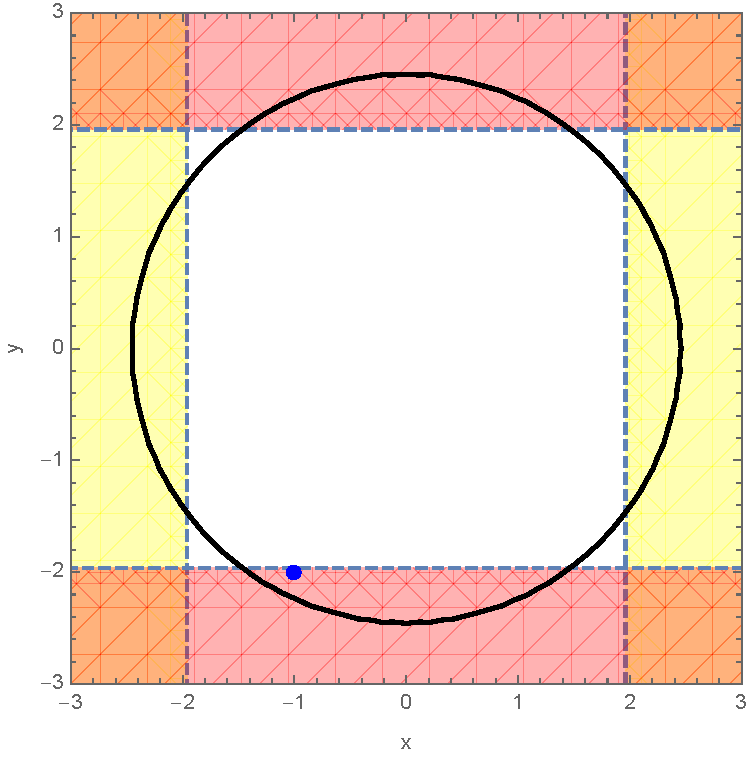
\includegraphics[width=.8\textwidth]{jointTtests1.pdf}	
\end{figure}
\end{column}
\begin{column}{0.5\textwidth}
\small{
If the $t$'s are independent:
\begin{itemize}
	\item The circle contains 95\% of the probability for two independent t-statistics;
	the area outside it is the rejection rejoin for the joint t-test.
	\item The dashed lines are the rejection regions for each of the individual t-tests.  (5\% level)
	\item Even though naively would reject, in actuality \emph{not significant}
	\item What happens with correlated normal RVs?
\end{itemize}
}
\end{column}

\end{columns}

\end{frame}

\begin{frame}{Bivariate normal: independent and correlated}
\begin{columns}
\begin{column}{0.5\textwidth}

	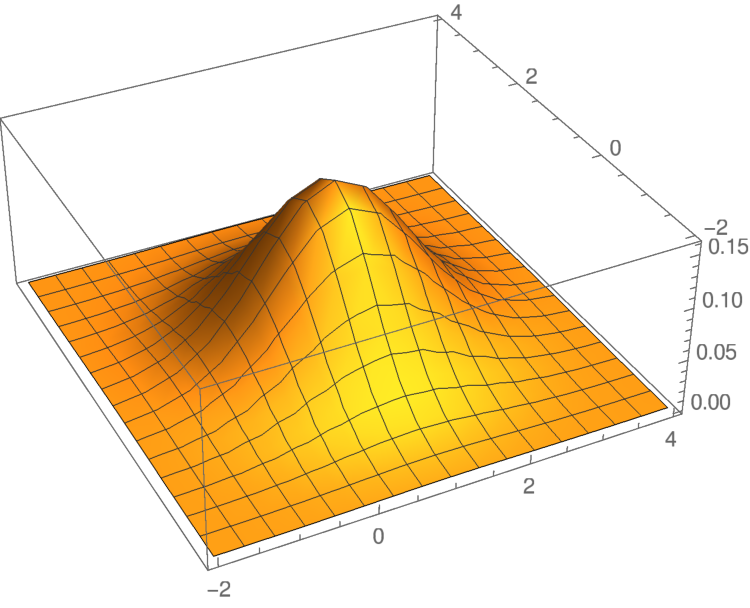
\includegraphics[width=1\textwidth]{joint_normal_ind.pdf}	
\end{column}
\begin{column}{0.5\textwidth}
	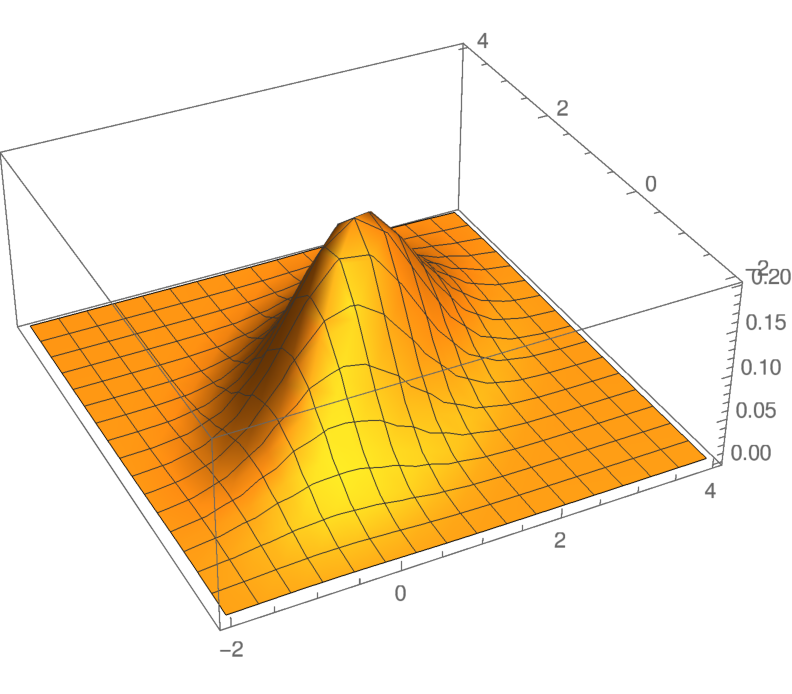
\includegraphics[width=1\textwidth]{joint_normal_corr.pdf}	
\end{column}

\end{columns}
	
\end{frame}


\begin{frame}{T-Tests with correlation}
\vspace{3mm}If the $t$'s are correlated this is the picture:
\begin{columns}
\begin{column}{0.5\textwidth}
\begin{figure}	
	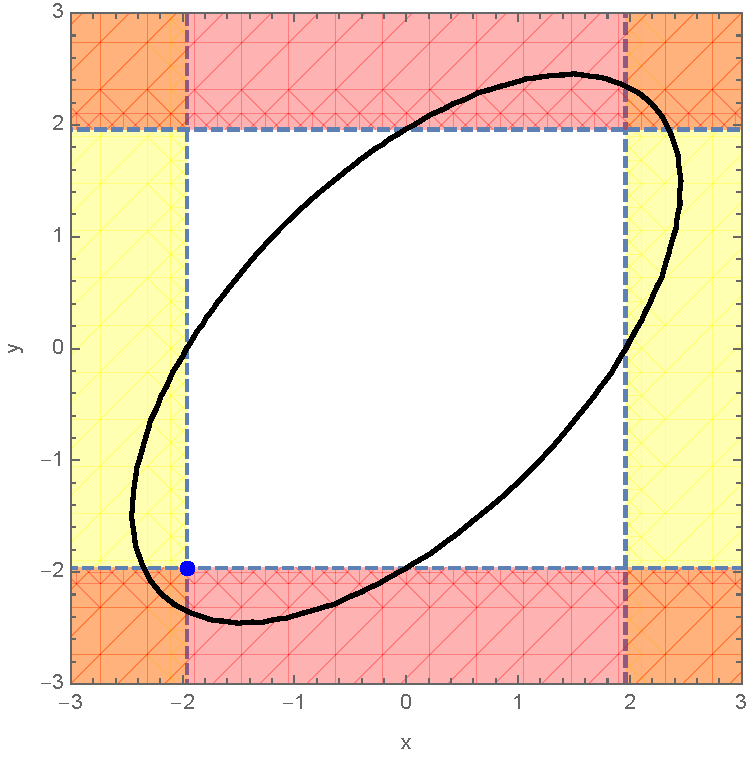
\includegraphics[width=.8\textwidth]{jointTtests2.pdf}	
\end{figure}
\end{column}
\begin{column}{0.5\textwidth}
\begin{itemize}
	\item Now, the area outside the ellipse is the rejection region for the joint t-test (5\% level)
	\item The dashed lines are the rejection regions for each of the individual t-tests.  (5\% level)
	\item Now, notice that even with $t_1 = -2$, $t_2=-2$, which would be a rejection according
	to each of the individual tests, is not a rejection of the joint test. 
\end{itemize}
\end{column}
\end{columns}

\end{frame}




\begin{frame}{Correcting for Correlation: The F-Test}

The issues we have are:
\begin{enumerate}
	\item Testing a joint hypothesis with independent tests will not give the correct type 1 error
	\item Correlated $\hat\beta$'s make things very messy	
\end{enumerate}

 How can we solve this?

\begin{itemize}
	\item First get a statistic that combines both hypotheses
		\begin{itemize}
			\item Should be ``big" when either $t_1$ or $t_2$ or both are big
			\item Should include both $t$'s
		\end{itemize}
	\item Natural candidate:
		\begin{align*}
			F = t_1^2 + t_2^2
		\end{align*}
	\begin{itemize}
		\item Always positive and only big when $t$'s are big
		\item If $t_1$ and $t_2$ are independent normals, then $F\sim \chi^2_2$
		\item If we divide by 2 we have $F_2$ distribution
	\end{itemize}
\end{itemize}	
\end{frame}

\begin{frame}{Correcting for Correlation: The F-Test, Cont'd}
Our candidate test:
	\[
		\frac{1}{2}\times (t_1^2 + t_2^2)
	\]

\begin{itemize}
	\item Has a well understood distribution \emph{when} $t$'s are independent
	\item If not, we can \emph{rotate} the $t$'s so they are
	\begin{itemize}
		\item Non-matrix formula (for 2 parameters):
		\[
			F = \frac{1}{2}\times\frac{t_1^2 + t_2^2 - 2\rho_{t_1,t_2}t_1t_2}{1-\rho_{t_1,t_2}}
		\]
		\item Matrix version (for $k$ parameters):
		\[
			\hat\beta-\beta\sim\mathcal{N}\left(0,\Sigma_{\hat\beta}\right)\Rightarrow \Sigma_{\hat\beta}^{-1/2}\times\left(\hat\beta-\beta\right)\sim\mathcal{N}(0,I)
		\]
		This implies,
		\[
		(\hat\beta-\beta)'\Sigma^{-1}(\hat\beta-\beta)/k\sim\chi^2_k/k = F_k
		\]
		
		
	\end{itemize}	
\end{itemize}	
\end{frame}

\begin{frame}{What is the F Distribution?}
New test statistic:
		\[
			F = \frac{1}{2}\times\frac{t_1^2 + t_2^2 - 2\rho_{t_1,t_2}t_1t_2}{1-\rho_{t_1,t_2}}
		\]

\begin{itemize}
	\item Almost always requires a computer
	\item Ugly formula that follows a simple distribution
	\item In general, for $q$ restrictions, we will calculate the $F$ statistic and it will be distributed $F_q$ ($F_{q,\infty}$ sometimes)
	\item Related to take the sum of squared normal random variables
	\item Critical values will depend on the number of restrictions
	\item Fun fact: for 1 restriction $F = t^2$
\end{itemize}

	
\end{frame}

\begin{frame}{Critical Values of the F}

\begin{figure}
\centering
	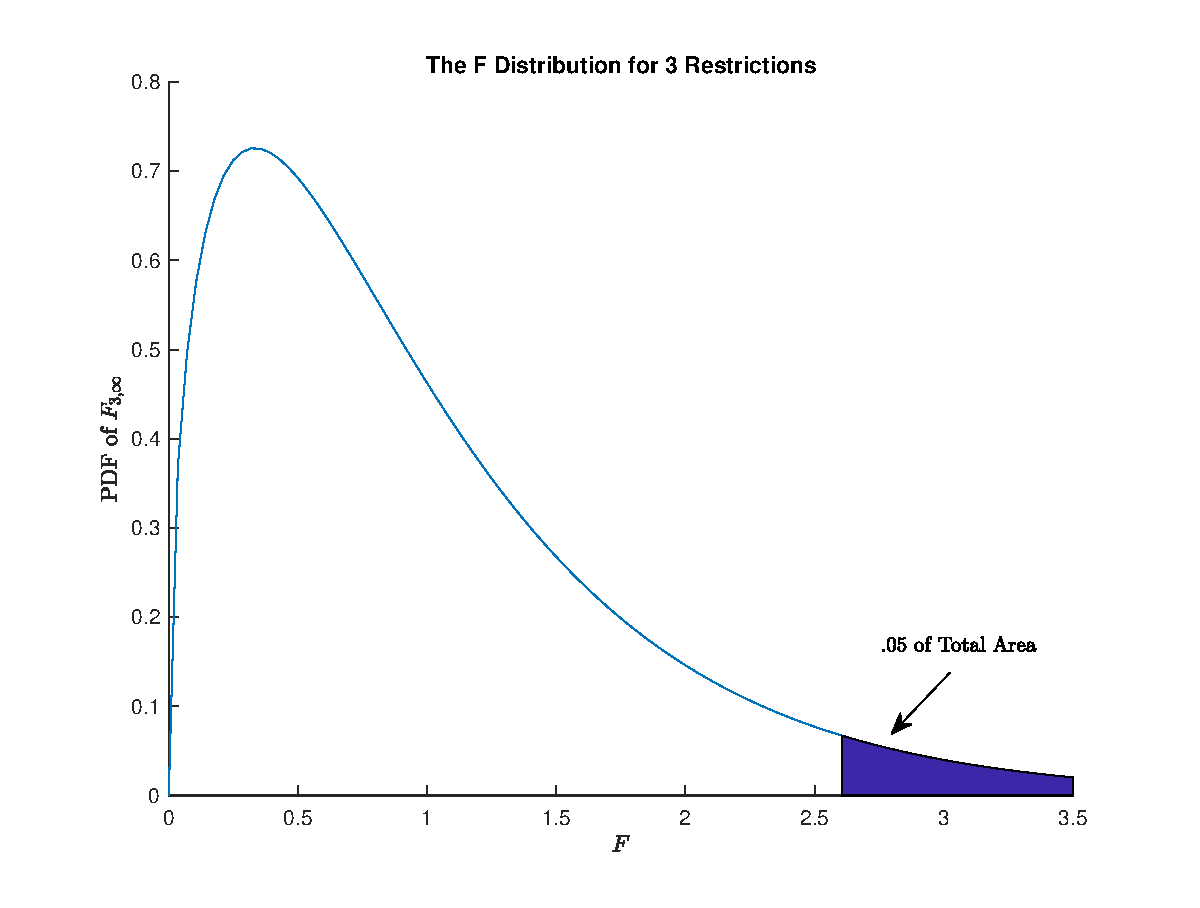
\includegraphics[width=.45\textwidth]{fDistributionk3.eps}	
\end{figure}

\vspace{-5mm}

\begin{itemize}
	\item The distribution looks different than the $t$
	\item But the testing procedure is the same!
	\begin{itemize}
		\item Find a critical value so that $P(F>cv)=.05$
		\item If $F$ is large \emph{given the null} then null is unlikely to be true
		\item Critical value depends on number of restrictions, $q$
	\end{itemize}	
\end{itemize}

\end{frame}




\begin{frame}{F-tests: General Definition}
\begin{itemize}
	\item We are interested in testing the following linear restrictions on the parameters:\[
	{\bf R} \boldsymbol{\beta} = {\bf q}, 
	\]
	where usually $ {\bf q} = {\bf 0}$, but not always.

	\item What would ${\bf R}$ and ${\bf q}$ be if we were testing whether two slopes were equal?

	\item The F statistic (or feasible Wald statistic):\[
F=\frac{\left(\boldsymbol{R}\boldsymbol{b}_{OLS}-\boldsymbol{q}\right)'\left\{ \boldsymbol{R}\left[s^{2}\left(\boldsymbol{X}'\boldsymbol{X}\right)^{-1}\right]\boldsymbol{R}'\right\} ^{-1}\left(\boldsymbol{R}\boldsymbol{b}_{OLS}-\boldsymbol{q}\right)}{J},
\]
which has a $F\left[J,n-K\right]$ distribution, where $J$ is the number of rows of ${\bf R}$ (the number of restrictions).

\end{itemize}
\end{frame}

\begin{frame}{F-tests: equivalent definitions}
\[
F=\frac{\left(\boldsymbol{R}\boldsymbol{b}_{OLS}-\boldsymbol{q}\right)'\left\{ \boldsymbol{R}\left[s^{2}\left(\boldsymbol{X}'\boldsymbol{X}\right)^{-1}\right]\boldsymbol{R}'\right\} ^{-1}\left(\boldsymbol{R}\boldsymbol{b}_{OLS}-\boldsymbol{q}\right)}{J},
\]
\begin{itemize}
	\item We could also write:\[
		F = \frac{SSE_{CLS} - SSE_{OLS}}{Js^2},
	\]
	where $SSE_{OLS}$ is the sum of squared residuals for the (unrestricted) OLS estimator, $SSE_{CLS}$
	is the sum of squared residuals under the {\bf constrained least squares} estimator with constraints ${\bf R} \boldsymbol{\beta} = {\bf q}$.

	\item We are not going to delve into constrained least squares, but the point here is that there are two equivalent ways to think about
	the F-statistic: (1) as a Wald statistic, which is based on comparing an asymptotically normal parameter estimate to a hypothesized value, 
	and (2) as an assessment of how much better the unconstrained model fits than the constrained model. 
\end{itemize}
\end{frame}





\begin{frame}{Non-Nested Models}
\begin{itemize}
	\item We have considered only nested models thus far. When testing \[
	{\bf R} \boldsymbol{\beta} = {\bf q}, 
	\]
	we are testing a restricted linear model against alternative hypothesis of 
	an unrestricted linear model, \emph{ which includes the restricted model as a special
	case}.

	\medskip
	\item Sometimes we want to compare non-nested models, which brings us to
	model selection. The main idea
	is to balance the model's goodness of fit and number of parameters: see
	adjusted $R^2$, {\bf Akaike Information Criterion}, {\bf Bayesian
	Information Criterion}. Machine learning approaches typically
	try to compare models by directly assessing out-of-sample performance.
	 More on this stuff later and/or next semester.

\end{itemize}
\end{frame}





%\begin{frame}{Confidence Intervals}
%\begin{itemize}
%	\item
%\end{itemize}
%\end{frame}



\begin{frame}{Confidence Intervals I}
\begin{itemize}
	\item Note that if 	\[
		{\bf b} \sim\mathcal{N}\left(\boldsymbol{\beta},\Sigma\right),
	\]
	then \[
		b_{k} \sim\mathcal{N}\left(\beta_k,\Sigma_{kk}\right),	
	\]
	and \[
	\Pr\left[ b_{k} - \alert{\underbrace{z_{\left(1-\alpha/2\right)}}_{1.96}} \sqrt{\Sigma_{kk}} \le \beta_k \le b_k +  \alert{\underbrace{z_{\left(1-\alpha/2\right)}}_{1.96}}  \sqrt{\Sigma_{kk}}  \right] =\alpha 
	\]
	where $ z_{\left(1-\alpha/2\right)} $ is the value such that the CDF of the standard normal distribution is $1-\alpha/2$. 	

\end{itemize}
\end{frame}




\begin{frame}{Confidence Intervals II}
\begin{itemize}
	\item Similarly, when \[
		\frac{b_k - \beta_k}{\sqrt{\hat{\Sigma}_{kk}}} \sim t_{n-K}
	\]
	because the variance $\Sigma_{kk}$ has to be estimated, then
 \[
	\hspace*{-1cm} \Pr\left[ b_{k} - \alert{t_{\left(1-\alpha/2\right),n-K}} \sqrt{\hat{\Sigma}_{kk}} \le \beta_k
	 \le b_k +  \alert{t_{\left(1-\alpha/2\right),n-K}}  \sqrt{\hat{\Sigma}_{kk}}  \right] =\alpha 
	\]
	where $ t_{\left(1-\alpha/2\right),n-K} $ is the value such that the CDF of the t-distribution with $n-K$ degrees of freedom is $1-\alpha/2$. 	

\end{itemize}
\end{frame}



\begin{frame}{Confidence Intervals III}
\begin{itemize}
	\item We define the $1-\alpha$ {\bf confidence interval} for $b_{k}$ as \[
	\left(b_{k} - t_{\left(1-\alpha/2\right),n-K} \sqrt{\hat{\Sigma}_{kk}} , b_k +  t_{\left(1-\alpha/2\right),n-K}  \sqrt{\hat{\Sigma}_{kk}} \right)
	\]

	\smallskip
	\item Note that this confidence interval is a function of the data -- the end points of the confidence interval 
	are statistics and therefore random variables in their own right. 

	\smallskip
	\item Defining the confidence interval in this way, the probability that the confidence interval contains
	the true parameter (\alert{coverage}) is $1-\alpha$ (if the asymptotic distribution of the estimator is taken as the true distribution). 
	That is, if $\alpha=.05$, this is called a 95\% confidence interval, and there
	is a 95\% chance it will contain the true parameter (assuming that the asymptotic approximation holds). 

\end{itemize}
\end{frame}


\begin{frame}{Bootstrap}
\begin{itemize}
\item Bootstrap takes a different approach.
\begin{itemize}
\item Instead of estimating $\hat{\theta}$ and then assuming a Normal/t-distribution
\item What if we directly tried to construct the \alert{sampling distribution} of $\hat{\theta}$?
\end{itemize}
\item Our data $((X_1,Y_1),\ldots,(X_n,Y_n)) \sim P$ are drawn from some measure $P$
\begin{itemize}
\item We can form a \alert{nonparametric estimate} $\hat{P}$ by just assuming that each $(X_i,Y_i)$ has weight $\frac{1}{n}$.
\item We can then simulate a new sample $(X^{*},Y^{*}) = ((X_1^{*},Y_1^{*}),\ldots, (Y_n^{*}, X_n^{*})) \sim \hat{P}$.
\begin{itemize}
\item Easy: we take our data and construct $n$ observations by \alert{sampling with replacement} 
\end{itemize}
\item Compute whatever statistic of $S(X^*,Y^*)$ we would like.
\begin{itemize}
\item Could be the OLS coefficients $\beta_1^{*},\ldots, \beta_k^{*}$.
\item Or some function $\beta_1^{*}/\beta_2^{*}$.
\item Or something really complicated: estimate parameters of a game $\hat{\theta}^*$ and now find Nash Equilibrium of the game $S(X^{*},Y^{*},\hat{\theta^*})$ changes.
\end{itemize}
\item Do this $B$ times and calculate at $Var(S_b)$ or $CI(S_1,\ldots, S_b)$.
\end{itemize}
\end{itemize}
\end{frame}


\begin{frame}{Bootstrap: Bias Correction}
\small
The main idea is that $\hat{\theta}^{1*},\ldots, \hat{\theta}^{B*}$ approximates the \alert{sampling distribution} of $\hat{\theta}$. There are lots of things we can do now:
\begin{itemize}
\item We already saw how to calculate $Var(\hat{\theta}^{1*},\ldots, \hat{\theta}^{B*})$.
\begin{eqnarray*}
\frac{1}{B-1} \sum_{b=1}^B (\hat{\theta}_{(b)}^* - \overline{\theta^{*}})^2
\end{eqnarray*}
\item Calculate $\E(\hat{\theta}^{*}_{(1)},\ldots, \hat{\theta}^{*}_{(B)}) = \overline{\theta^{*}} = \frac{1}{B} \sum_{b=1}^B \hat{\theta}_{(b)}^*$.
\end{itemize}
\end{frame}

\begin{frame}{Bootstrap: Bias Correction}
\begin{itemize}
\item We can use the estimated bias to \alert{bias correct} our estimates
\begin{eqnarray*}
Bias(\hat{\theta}) &=&\E[\hat{\theta}] - \theta \\
Bias_{bs}(\hat{\theta}) &=&\overline{\theta^{*}} -\hat{\theta}
\end{eqnarray*}
Recall $\theta = \E[\hat{\theta}] - Bias[\hat{\theta}]$:
\begin{eqnarray*}
\hat{\theta}- Bias_{bs}(\hat{\theta}) = \hat{\theta}-(\overline{\theta^{*}}-\hat{\theta}) = 2 \hat{\theta} - \overline{\theta^{*}}
\end{eqnarray*}
\item Correcting bias isn't for free - variance tradeoff!
\item Linear models are (hopefully) unbiased, but most nonlinear models are \alert{consistent but biased}.
\end{itemize}

\end{frame}

\begin{frame}{Bootstrap: Confidence Intervals}
There are actually three ways to construct bootstrap CI's:
\begin{enumerate}
\item Obvious way: sort  $\hat{\theta}^{*}$ then take $CI: [\hat{\theta}^{*}_{\alpha/2},\hat{\theta}^{*}_{1-\alpha/2}]$.
\item Asymptotic Normal:  $CI: \hat{\theta} \pm 1.96 \sqrt{V(\hat{\theta}^{*})}$. (CLT).
\item Better Way: let $W= \hat{\theta} -\theta$. If we knew the distribution of $W$ then: $Pr(w_{1-\alpha/2} \leq W \leq w_{\alpha/2})$:
\begin{eqnarray*}
CI: [\hat{\theta} -w_{1-\alpha/2}, \hat{\theta} -w_{\alpha/2}]
\end{eqnarray*}
We can estimate with $W^{*} = \hat{\theta}^{*} - \hat{\theta}$.
\begin{eqnarray*}
CI: [\hat{\theta} -w^*_{1-\alpha/2}, \hat{\theta} -w^*_{\alpha/2}] = [2 \hat{\theta} -\theta^*_{1-\alpha/2}, 2 \hat{\theta} -\theta^*_{\alpha/2}]
\end{eqnarray*}
Why is this preferred? Bias Correction!
\end{enumerate}

\end{frame}


\begin{frame}{Bootstrap: Why do people like it?}
\begin{itemize}
\item Econometricians like the bootstrap because under certain conditions it is \alert{higher order efficient} for the confidence interval construction (but not the standard errors).
\begin{itemize}
\item Intuition: because it is non-parametric it is able to deal with more than just the first term in the Taylor Expansion (actually an \alert{Edgeworth Expansion}).
\item Higher-order asymptotic theory is best left for real econometricians!
\end{itemize}
\item Practitioner's like the bootstrap because it is easy.
\begin{itemize}
\item If you can estimate your model once in a reasonable amount of time, then you can construct confidence intervals for most parameters and model predictions.
\end{itemize}
\end{itemize}
\end{frame}

\begin{frame}{Bootstrap: When Does It Fail?}
\begin{itemize}
\item Bootstrap isn't magic. If you are constructing standard errors for something that isn't asymptotically normal, don't expect it to work!
\item The Bootstrap exploits the notion that your sample is IID (by sampling with replacement). If IID does not hold, the bootstrap may fail (but we can sometimes fix it!).
\item Bootstrap depends on asymptotic theory. In small samples weird things can happen. We need $\hat{P}$ to be a good approximation to the true $P$ (nothing missing).
\end{itemize}
\end{frame}

\begin{frame}{Bootstrap: Variants}
The bootstrap I have presented is sometimes known as the \alert{nonparametric bootstrap} and is the most common one.
\begin{description}
\item[Parametric Bootstrap] ex: if $Y_i = \beta_0 + \beta_1 X_i + \epsilon_i$ then we can estimate $(\hat{\beta}_0,\hat{\beta}_1)$ via OLS.\\
 Now we can generate a bootstrap sample by drawing an $x_i$ at random with replacement $\hat{\beta}_0 + \hat{\beta}_1$ and then drawing \alert{independently} from the distribution of estimated residuals $\hat{\epsilon}_i$.
 \item[Wild Bootstrap] Similar to parametric bootstrap but we rescale $\epsilon_i$ to allow for \alert{heteroskedasticity}
\item[Block Bootstrap] For correlated data (e.g.: time series). Blocks can be overlapping or not.  
\end{description}
\end{frame}


\begin{frame}{Summary}
\begin{itemize}
	\item Linear regression theory gives us formulas for estimating $Var\left({\bf b}_{OLS}\right)$

	\item We can use that variance estimator to test hypotheses about parameters (using t-Tests
	and f-Tests) as well as construct confidence intervals. 

	\item When the baseline assumptions of the linear regression model are violated (due to
	correlation or heteroscedasticity), we need to use somewhat more complex formulas
	to estimate  $Var\left({\bf b}_{OLS}\right)$.

\end{itemize}
\end{frame}



\end{document}